\section{Mission Analyses}
\f{Earth-Synchronous Orbit}
\begin{itemize}
 \item the ground track repeats after a specific period of time
 \item Earth's rotation rate is the sidereal rotation period = sidereal day $\uptau_{\text{\tiny{E}}}$
 \item $\uptau_E$ is varying with time $\uptau_E = 86164.10555+0.15\cdot C$ [s] where C is the centuries since year 2000
 \item as the Earth rotates eastward, the satellite is thus moving relative to the surface in westward direction by 
 \[\Delta \Phi_r = 2\pi\frac{T}{\uptau_{\text{\tiny{E}}}} \text{ [rad/rev]}\] 
 \item second effect influencing the shift of the subsatellite point is the rotation of the satellite's orbit plane $\Delta \Omega$
 \item as $\Delta \Omega$ is positive in eastward direction, these two effects are combined to the total angular shift $\Delta \Phi$ at subsequent equator 
 passages \[\Delta \Phi = \Delta \Phi_r - \Delta \Omega \text{ [rad/rev]}\]
 \item to be Earth-Synchronous: 
 \[n\Delta \Phi = m \cdot 2\pi\]
\end{itemize}
\f{Sun-Synchronous Orbit}
\begin{itemize}
 \item die Erde braucht $\uptau_S = 3.155815\cdot 10^7 s$, um einmal um die Sonne zu kreisen 
 \item bei einem sonnensynchronen Orbit muss der Winkel zwischen Sonnenrichtung und Orbitebene konstant bleiben 
 \item also muss sich die Ebene pro Tag um einen Winkel $\theta$ drehen 
 \[\theta = 2\pi\frac{\uptau_{\text{\tiny{E}}}}{\uptau_{\text{\tiny{S}}}} \text{ [rad/day]} = 2\pi\frac{\uptau_{\text{\tiny{E}}}}{\uptau_{\text{\tiny{S}}}}\frac{T}{\uptau_{\text{\tiny{E}}}} \text{ [rad/rev]}\]
\end{itemize}
\f{Earth- and Sun-Synchronous Orbit}
\begin{itemize}
 \item \[\Delta \Omega = \theta \Rightarrow T\left(\frac{1}{\uptau_{\text{\tiny{E}}}} - \frac{1}{\uptau_{\text{\tiny{S}}}}\right) = \frac{m}{n}\]
 \item angular shift between two subsequent orbits 
 \[\Delta \Phi = \Delta \Phi_r - \Delta \Omega = 2\pi T\left(\frac{1}{\uptau_{\text{\tiny{E}}}} - \frac{1}{\uptau_{\text{\tiny{S}}}}\right) \text{ [rad/rev]}\]
 worst case between subsequent orbits $\Delta \Phi \cdot R_E$.
\end{itemize}
\f{Eclipse periods}
angle between Earth-Sun vector and normal vector to orbit plane: $\sin \beta = \vec{s}\cdot\vec{n}$\\
Earth central angular radius at entry into eclipse: $\beta^* = \sin^{-1}\left(\frac{R_E}{h+R_E}\right)$\\
Angular arc of orbit in shadow: $2\cos^{-1}\left(\frac{\cos \beta^*}{\cos \beta}\right)$
\f{Ground Contact and Coverage Analyses}
altitude $h$, visible horizon characterized by angles $\rho$ and $\lambda_0$: $\rho + \lambda_0 = 90\degree$
\begin{align*}
 R_E &= (R_E + h) \cos \lambda_0\\
 &= (R_E +h) \sin \rho\\
\end{align*}
observe $\Lambda_t, \Theta_t$ (long,lat) from known orbit position of satellite, characterized by subsatellite point $\Lambda_s, \Theta_s$.\\
characteristic paramters:
\begin{itemize}
 \item nadir angle $\eta$
 \item earth central angle $\lambda$
 \item spacecraft elevation angle $\varepsilon$
\end{itemize}
\begin{figure}[!ht]
 \centering
 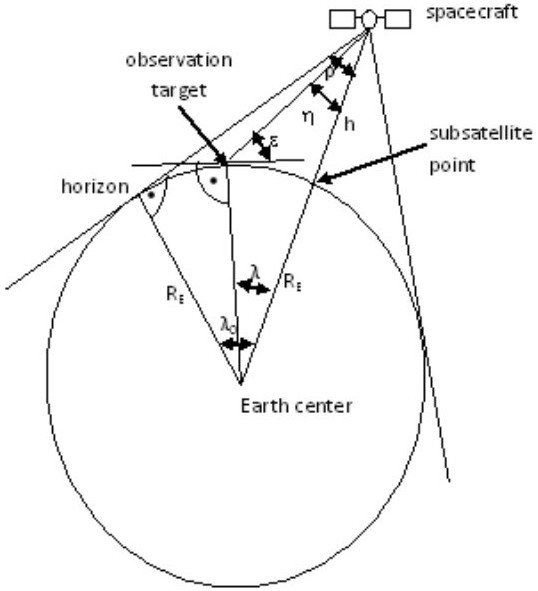
\includegraphics[scale=0.6]{groundcoverage}
\end{figure}
calculate nadir angle $\eta$:
\[ \tan \eta = \frac{\frac{R_E}{R_E+h}\sin \lambda}{1-\frac{R_E}{R_E+h}\cos\lambda}\]
\[ \lambda + \eta + \varepsilon = 90\degree \]
$\lambda_\text{max}$: maximum earth central angle $\Rightarrow$ swath width $2\lambda_\text{max}$ perpendicular to groundtrack on surface.\\
Time in view $T_\text{view}$ for circular orbit with period $T$:
\[ T_\text{view} = \frac{T}{180\degree}\cos^{-1}\left(\frac{\cos \lambda_\text{max}}{\cos \lambda}\right)\]
\f{ground station contact periods}
\begin{figure}[!ht]
 \centering
 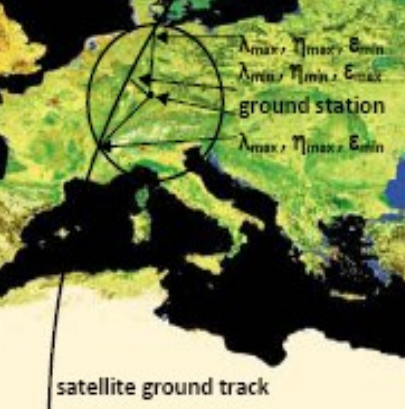
\includegraphics[scale=0.6]{groundtrack}
\end{figure}
\begin{itemize}
 \item $\sin\eta_\text{max} = \cos \varepsilon_\text{min}\frac{R_E}{R_E+h}$
 \item $\lambda_\text{max} = 90\degree - \varepsilon_\text{min} -\eta_\text{max}$
 \item max range satellite$\leftrightarrow$groundstation: $D_\text{max} = R_E\frac{\sin\lambda_\text{max}}{\sin\eta_\text{max}}$
 \item total time in view: $ T_\text{view} = \frac{T}{180\degree}\cos^{-1}\left(\frac{\cos \lambda_\text{max}}{\cos \lambda_\text{min}}\right)$
 \item contact only possible, if station-orbit angle $<$ central angle of contact cone
\end{itemize}

